\chapter{Introducing heterogeneities}
\label{chp:chp4}

In this chapter, we will consider how to mark, remove, and mesh
different regions of the brain and its environment based on
{\freesurfer} segmentations. We will
\begin{itemize}
\item
  Create hemisphere meshes differentiating between gray and white matter,
\item
  Create hemisphere meshes without ventricles,
\item
  Create brain meshes by combining the two hemispheres,
\item
  Map parcellations\footnote{A parcellation is a way of dividing the brain 
  into distinct regions. {\freesurfer}, for instance, does this as part of 
  the \emp{recon-all} process and this is why we can use Freeview to view the 
  different parts of a subject's brain, such as the hippocampus or anterior 
  cingulate, after \emp{recon-all} completes.} 
  onto brain meshes, and
\item
  Locally refine parcellated brain meshes.
\end{itemize}

\section{Hemisphere meshing with gray and white matter}
\label{sec:chp4:tools:gray-white}

Gray and white matter differ substantially in their
characteristics. These differences can often be represented in
mathematical models and simulations by differing material
properties. For instance, denoting the domains occupied by gray and
white matter by $\Omega_g$ and $\Omega_w$ respectively, we may want to
consider heterogeneous diffusion tensors in~\eqref{eq:diffusion}, for
example, such that
\begin{equation}
  \label{eq:K}
  D = D(x) = \left \{
    \begin{matrix}
      D_g & \quad x \in \Omega_g, \\
      D_w & \quad x \in \Omega_w 
    \end{matrix}
    \right .
\end{equation}
where $D_g$ and $D_w$ take on different values, and $D_g$ may be
scalar-valued and $D_w$ tensor-valued. To represent fields such as $D$
in numerical simulations, it is useful to transfer the information
about gray and white matter from the magnetic resonance (MR) images
into the meshes. To introduce the basic concepts of differentiating
brain regions, we will once more create a computational mesh of the left
hemisphere.  In Chapter~\ref{chp:chp3}, all of the mesh tetrahedrons belonged 
to a single region.  In this chapter, we extend the previous approach 
by creating a mesh where the individual tetrahedrons will be labeled as 
belonging to the gray matter, the white matter, or the ventricles. In short, 
we will
\begin{itemize}
\item
  Create STL files from the pial and white FreeSurfer left hemisphere
  surfaces, 
\item
  Create a mesh from these STL files conforming to the interior interfaces
  between white and gray matter, using \svmtk{}, and
\item
  Include tags for different regions of the mesh.  That is, for each 
  tetrahedron in the mesh we want to label it as residing in the 
  `gray matter', `white matter', `ventricles', etc.     
\end{itemize}

\subsection{Converting pial and gray/white surface files to STL}
\index{FreeSurfer}
\index{FreeSurfer!\emp{mris\_convert}}
Starting with the \freesurfer{} segmentation and using the book data
from \emp{freesurfer/ernie/surf/} as an example, we first convert the
left hemisphere pial surface (\emp{lh.pial}) and gray-white interface
surface (\emp{lh.white}) files to the STL format (as described in
Chapter~\ref{sec:chp3:surfaces}):
\terminal{\$ mris\_convert ./lh.pial pial.stl\\
\$ mris\_convert ./lh.white white.stl
}
\noindent We can now also improve the quality of the resulting
surfaces as discussed in
Chapter~\ref{sec:chp3:improved-volume-meshing}\footnote{We leave the
  precise code for this as an exercise for the reader. The resulting
  files could be called \emp{lh.pial.smooth.stl} and
  \emp{lh.white.smooth.stl}, respectively. For simplicity, we assume that the
  resulting pial and white surface STL files are (re)named
  \emp{lh.pial.stl} and \emp{lh.white.stl}, respectively, in the following. As 
  noted in Chapter~\ref{chp:chp3}, the automatic addition of the prefix lh., in
  lh.pial.stl, can be avoided by using ./ in the output filename.}.

\subsection{Creating the gray and white matter mesh}%
\label{sec:chp4:tools:gray-white:mesh-creation}
\index{SVM-Tk!\emp{Domain}}
\index{SVM-Tk!\emp{SubdomainMap}}
\index{ParaView}
Given these two surfaces, we can create a volume mesh conforming to
the interior (gray--white) surface, with the white and gray regions
identified separately. We will use \svmtk{} for this task, and
proceed with an \svmtk{} code example. We will wrap the main
functionality in a Python function
\pythoninline{create\_gw\_mesh}. This function can then, for instance,
be called as
\newpythonsnippet{chp4}{two-domain-tagged.py}{25}{28}
to use the two STL surface files from above as input and create a new
file \emp{ernie-gw.mesh} for the resulting volume mesh.

Our function first loads the two surfaces using \svmtk{}:
\newpythonsnippet{chp4}{two-domain-tagged.py}{0}{8}

\noindent Notice that the list \pythoninline{surfaces = [pial, white]} contains 
two surfaces; the order of these surfaces in this list will matter.  We next 
create a tailored \svmtk{} \pythoninline{SubdomainMap} object that represents 
a map between regions defined by surfaces and tags. This map is defined by
(repeated) calls to \emp{smap.add} with a string representing the
region and an integer representing the tag as arguments. The (binary)
string is a sequence of zeros and ones, with zero denoting the outside
and one the inside\footnote{Note that the STL surface 
format includes information about the orientation of the surfaces via the 
surface normals: each surface thus has an orientation, with an inside and an 
outside direction.}.
\newpythonsnippet{chp4}{two-domain-tagged.py}{9}{14}

Intuitively, \pythoninline{smap.add("10",1)} will mean `those tetrahedron 
inside surface 1 (pial surface) and outside surface 2 (white matter surface) 
should be marked with the numeric (tag) value of 1' while 
\pythoninline{smap.add("11",2)} will mean `those tetrahedron inside surface 1 
(pial surface) and inside surface 2 (white matter surface) should be marked 
with the numeric (tag) value of 2'.  At this point, however, \svmtk{} does not 
know that the \pythoninline{surfaces} list and our 
\pythoninline{SubdomainMap} object, \pythoninline{smap}, are related.  Relating 
a surface list to a \pythoninline{SubdomainMap} object is handled by creating 
a \pythoninline{Domain} object; a \pythoninline{Domain} object is constructed  
from the ordered list of surfaces and the subdomain map as follows:
%
%An \svmtk{} \pythoninline{Domain} object can be constructed from the
%ordered list of surfaces and the subdomain map:
%
\newpythonsnippet{chp4}{two-domain-tagged.py}{16}{19}

%\noindent Note that the \pythoninline{Domain} object here links the
%surfaces and the subdomain map. 
\noindent The \pythoninline{Domain} object reads the entries, registered above 
as \pythoninline{smap.add("10",1)} etc, of the 
\pythoninline{SubdomainMap} with respect to the ordering of the entries in 
our \pythoninline{surfaces} list.  The important point here is that the 
order of the entries in the \pythoninline{surfaces} list plays a key role; 
permuting the entries will yield different results.  % 
%The order of the entries in the list
%of surfaces is matched to the binary region strings in the subdomain
%map. 
For the code above, the string \pythoninline{"10"} %referring to the list \pythoninline{[pial, white]} 
is interpreted as `inside pial' and `outside white' and thus represents all 
tetrahedron in the region between the pial and white surface; this region 
consists of only the gray matter. Similarly, the string \pythoninline{"11"} is 
interpreted as 'inside pial' and 'inside white' and thus represents all 
tetrahedron in the white matter region since this region lies within both 
surfaces.  %
%
%region inside the gray--white surface, that
%is, the white matter. 
We will discuss \pythoninline{SubdomainMap} further in 
Chapter~\ref{chp4:subdomains} below.

With \pythoninline{domain}, we can now create a volume mesh of
suitable resolution and save it in the .mesh format (as in
Chapter~\ref{subsec:chp3:mesh-creation}):
\newpythonsnippet{chp4}{two-domain-tagged.py}{20}{24}
This script is also available as \emp{mri2fem/chp4/two-domain-tagged.py} in the
book scripts, and can be run from there as:
\terminal{\$ python two-domain-tagged.py}
\index{meshio!\emp{meshio-convert}}
\noindent As before, the resulting \emp{.mesh} file can be converted to different formats
using meshio. For instance, to convert to the ParaView-friendly .vtu format, use:
\terminal{\$ meshio-convert ernie-gw.mesh ernie-gw.vtu}

We used ParaView to visualize the tags associated with this mesh
in Figure~\ref{fig:chp4:ernie-tagged-twodomain-mesh}.  To see a view similar 
to that of Figure~\ref{fig:chp4:ernie-tagged-twodomain-mesh} in ParaView, first 
load \emp{ernie-gw.vtu} by selecting \button{File$\rightarrow$Open} and s
electing \emp{ernie-gw.vtu}, then click \button{Apply} to show the mesh.  In 
the left-hand window, under the \emp{Coloring} heading, select the second 
entry titled \emp{medit:ref}.  Now select 
\button{Filters$\rightarrow$Alphabetical$\rightarrow$Clip} from the top menu 
bar.  The clipping plane should, by default, appear in the middle of the mesh 
with the (red) clipping plane in the sagittal orientation.  Click the 
\button{Apply} button in the left-hand window to cut the mesh and reveal the 
tagged gray and white matter (tagged) tetrahedron.  We see that the
mesh cells associated with the gray matter region have the value 1,
while the cells associated with the white matter region have the value
2, as defined by our subdomain map.

\begin{figure}
  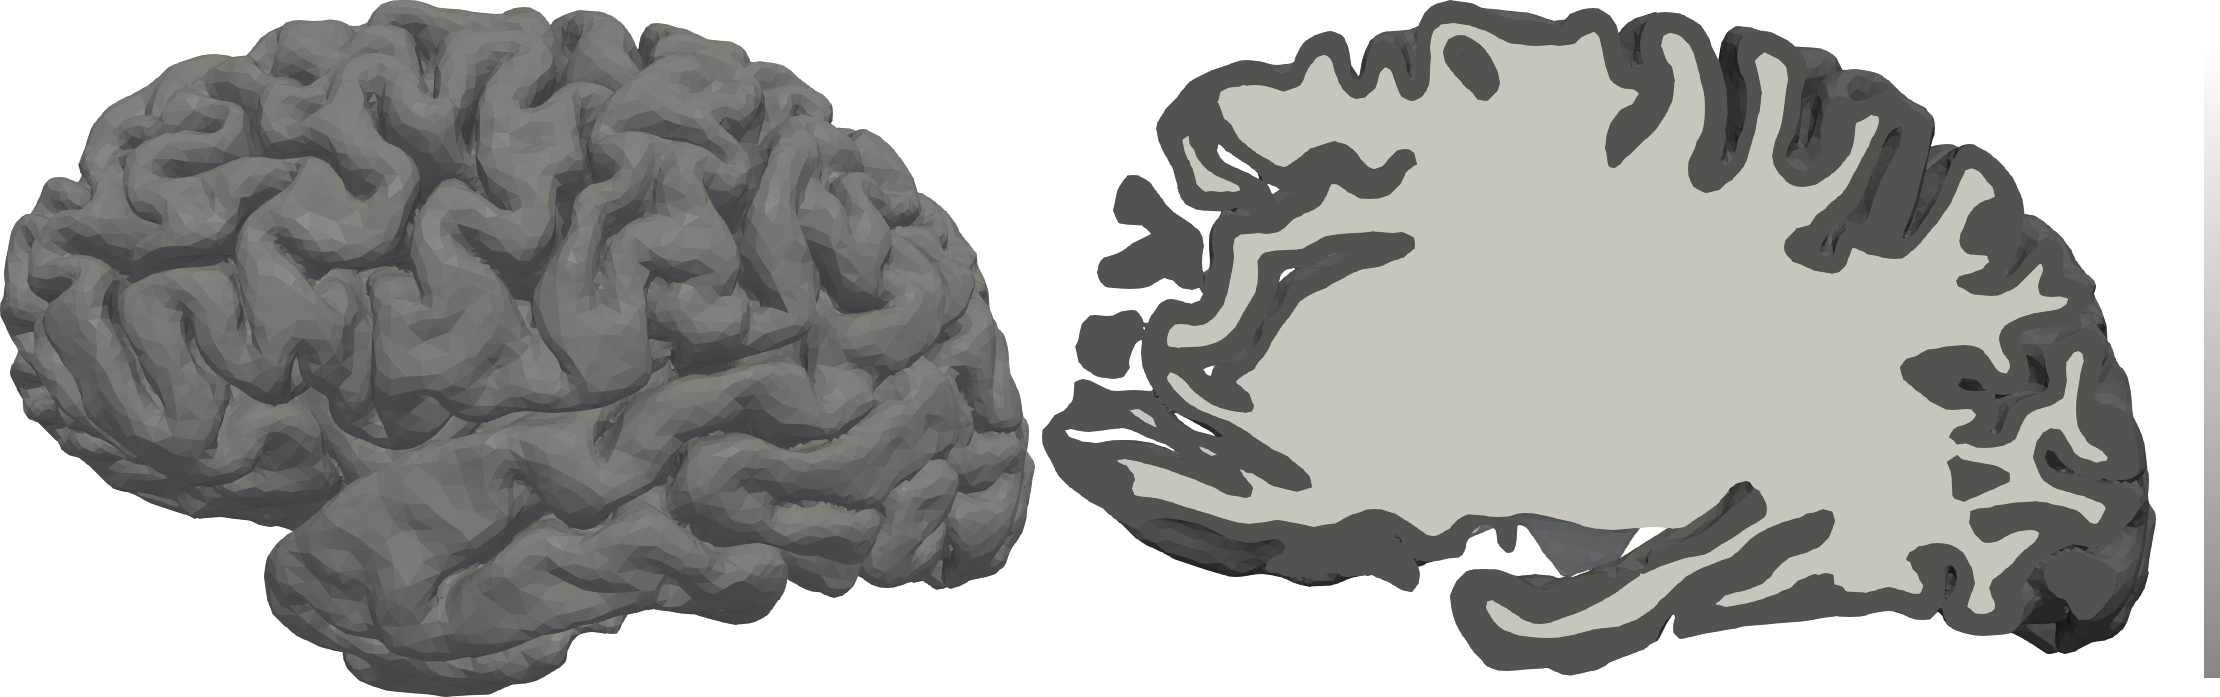
\includegraphics[width=0.99\textwidth]{./graphics/chp4/two-domain-tagged-bw.png}
  \caption{Volume mesh of the left hemisphere conforming to the
    interior gray--white interface.  Gray matter is tagged with a value of 1 
    and white matter is tagged with a value of 2.  The color scale is inverted. 
    A sagittal view (left) of the left hemisphere volume mesh and a sliced 
    (right) view exposes the interior white matter region.}
  \label{fig:chp4:ernie-tagged-twodomain-mesh}
\end{figure}

As a side note, we observe that the ventricles have been labeled as
white matter (see Figure \ref{fig:chp4:ernie-tagged-twodomain-mesh},
right), since the ventricles are positioned inside the gray--white
interface surface. Removal of the ventricles from our computational mesh
is the topic of Chapter~\ref{sec:chp4:tools:remove-vent}.

\subsection{More about defining \svmtk{} subdomain maps}  
\label{chp4:subdomains}
\index{SVM-Tk!\emp{SubdomainMap}}
To provide more detail about the \svmtk{} feature
\pythoninline{SubdomainMap}, we consider another, more involved
example. We now assume that we have four surfaces: a left pial
surface, a right pial surface, the whole white matter surface and a
surface enclosing the ventricles. A schematic of this set-up is
illustrated in Figure~\ref{fig:chp4:smap-example}. Now, let us see how
we can tag all the tetrahedra of the ventricles.
\begin{figure}[t]
  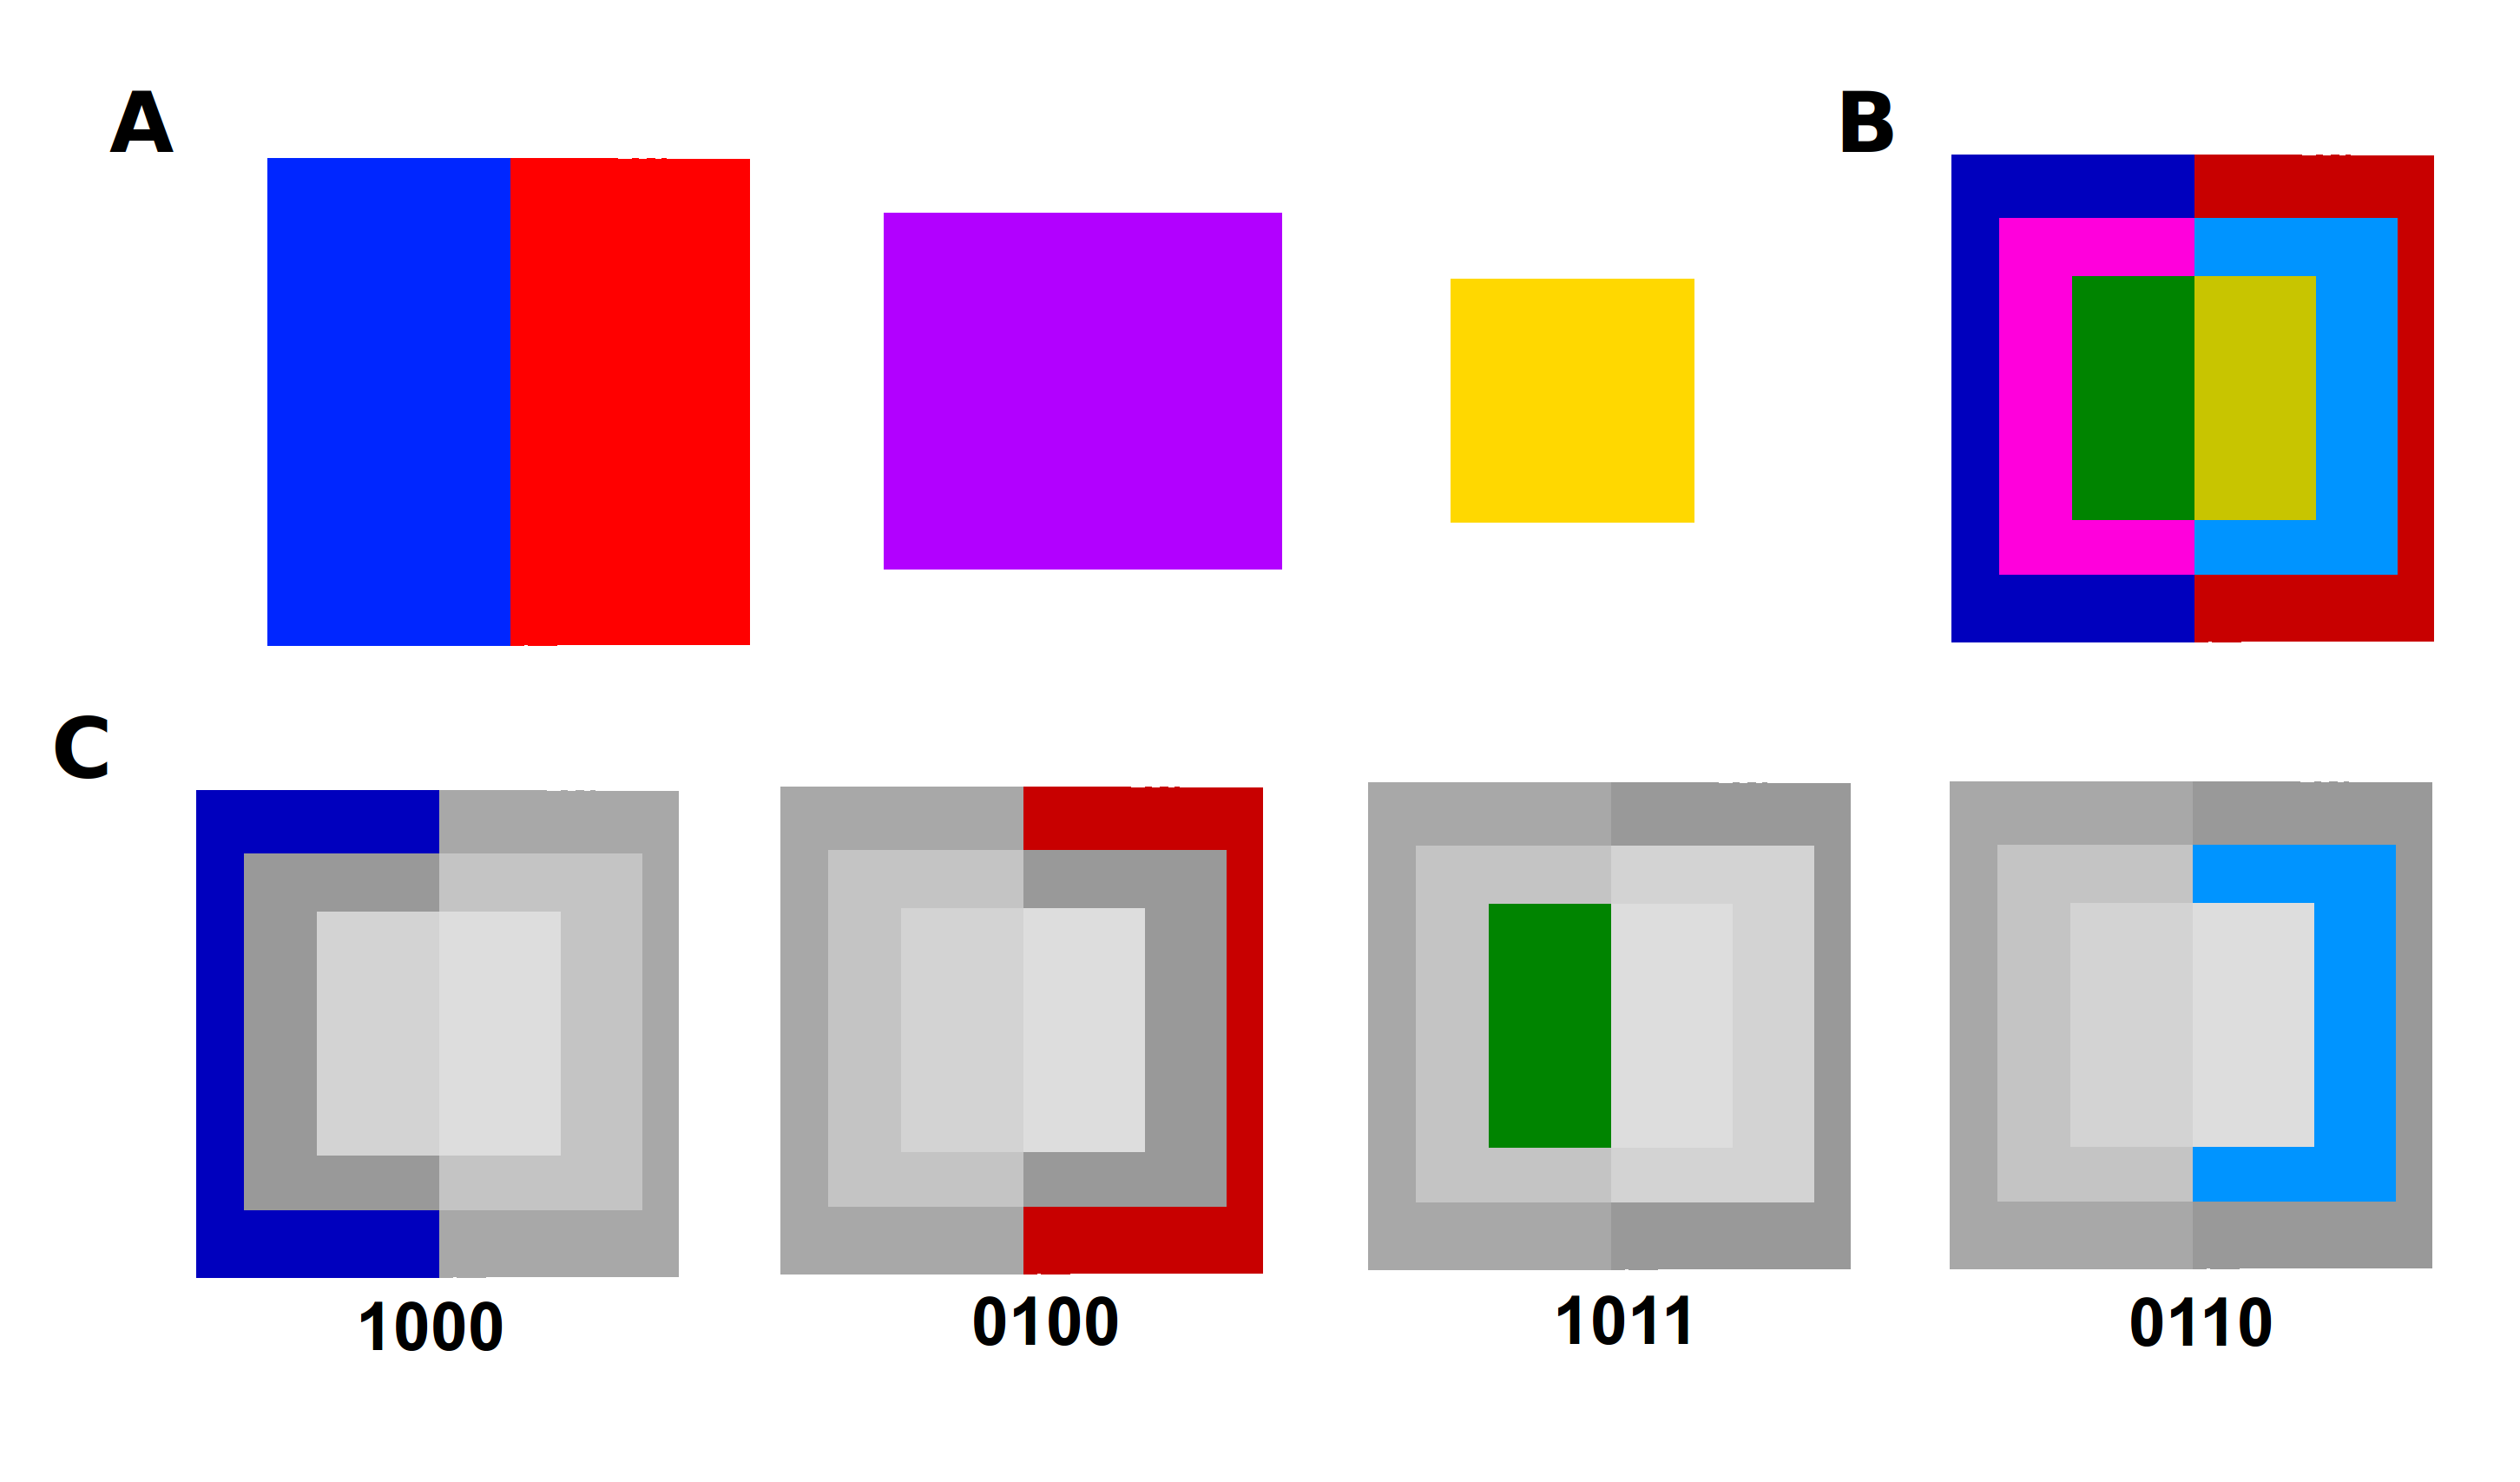
\includegraphics[width=0.95\textwidth]{./graphics/chp4/dot.png}
%  \caption{The upper left panel, A), shows colored squares, each
%    schematically representing a domain enclosed by a surface. The
%    left hemisphere is blue, the right hemisphere is red, the white
%    matter is purple, the ventricles are yellow, and their bounding
%    surfaces are given in this order. The upper right panel B) shows the
%    combination of each colored square. The bottom panel C) shows four
%    different subdomains and its corresponding bit-string. The left
%    image, 1000, denotes the volume that is within the left
%    hemisphere, but not within the right hemisphere, white matter or
%    ventricles -- hence the gray matter of the left hemisphere. The
%    image 0100 is completely analogous for the right hemisphere. Then
%    1011 refers to the surface that is within the left hemisphere
%    and within both the white surface and ventricles; hence the left
%    ventricle. Finally, 0110 represents the white matter of the
%    right hemisphere. }
  \caption{The upper left panel, (A), shows three colored squares that 
	differentiate the volumes enclosed by the large scale surfaces 
	files, in the \pythoninline{surfaces} list, at their simplest level.  
	The left hemisphere volume is colored blue, the right hemisphere volume 
	is colored red, the white matter volume is purple and the ventricle 
	volume is yellow.  The upper right panel (B) shows the complex 
	combination of volumes that can be separately tagged using 
	\pythoninline{smap.add} and the surfaces defined in the 
	\pythoninline{surfaces} list.  The regions of (B) are colored by an 
	independent color scheme that shows all possible combinations, of 
	volumes, addressable by \pythoninline{smap.add}.  The bottom panel (C) 
	shows four, of the six, different subdomains of (B) and their corresponding bit 
	strings. The left image, corresponding to bit string `1000', denotes 
	the volume that is within the left hemisphere, but not within the right 
	hemisphere, white matter or ventricles -- hence the gray matter of the 
	left hemisphere.  The image with bit string `0100' is completely 
	analogous for the right hemisphere. The bit string `1011' refers to the 
	surface that is within the left hemisphere and within both the white 
	surface and ventricles; hence the left ventricle. Finally, the image 
	for the bit string `0110' corresponds to the white matter of the right 
	hemisphere. For completeness, the remaining two bit strings for the 
	regions shown in (B) are `1010' (left, magenta region) and `0111' 
	(right, golden region).}
\label{fig:chp4:smap-example}
\end{figure}

To represent the subdomains, assuming that \pythoninline{lpial, rpial,
  white}, and \pythoninline{ventricles} exist as
\pythoninline{svmtk.Surface}s, we could use the following sample code:
\begin{python} 
surfaces = [lpial, rpial, white, ventricles]
smap = svmtk.SubdomainMap()
\end{python}
The ventricles are filled with cerebrospinal fluid.  A practical motivation for 
tagging the ventricles separately may be, for example, a desire to specify a 
much faster (isotropic) diffusion coefficient in the ventricular domain.  Here, 
we demonstrate the marking all of the mesh tetrahedrons that lie inside the 
subdomain defined by the ventricle surface with a (tag) value of 6. To do this, %
%To mark all the tetrahedra in the ventricles in the left hemisphere
%with the tag value 6, 
%we need to identify the placement of the left ventricles within the ordered 
%list of surfaces
we need to identify the placement of volume corresponding to the left 
ventricles; as we have seen, this volume is defined implicitly by the surfaces 
within the list \pythoninline{surfaces}.  The ventricles in the left hemisphere are inside the left 
pial surface, outside the right pial surface, inside the gray-white matter 
surface and inside the ventricular surface, resulting in the bit-string "1011". 
We could thus call \pythoninline{smap.add} as 
\begin{python}
smap.add("1011", 6)
\end{python}
Similarly, we can tag the ventricle volume within the right pial
surface by
\begin{python}
smap.add("0111", 6)
\end{python}
Finally, we can tag the ventricular volume at the intersection of the
left and right pial surfaces via
\begin{python}
smap.add("1111", 6)
\end{python}
Indeed, tagging the entire ventricular volume in this manner requires that we add all
three of the lines above.

Finally, we note that {\svmtk} also allows for marking several
domains at once:
\begin{python}
smap.add("10*", 6)
\end{python}
will mark all underlying domains, that is, in this case "1000", "1001",
"1010", and "1011".  Note that the use of the asterisk requires a
prior specification of the number of input surfaces, either as an
optional argument in the constructor, of a \pythoninline{SubdomainMap} object 
such as \pythoninline{smap}, or by using the member function 
\pythoninline{set\_number\_of\_surfaces} of the \pythoninline{SubdomainMap} 
class (for example,  \pythoninline{smap.set\_number\_of\_surfaces}). Therefore, 
as an alternative, one could just include the line
\begin{python}
smap.add("*1", 6)
\end{python}
instead of adding each ventricular volume separately.

\section{Separating the ventricles from the gray and white matter}
\label{sec:chp4:tools:remove-vent}

The volume hemispheric meshes created in Chapter~\ref{chp:chp3}, and the
volume hemisphere mesh illustrated in 
Figure~\ref{fig:chp4:ernie-tagged-twodomain-mesh} include the
ventricles as part of the white matter. Since the physics of the
fluid-filled ventricles and the soft but solid brain cerebrum may be
very different, removal of the ventricles from the hemisphere volume
is a useful operation. Here, we demonstrate how to (i) use
{\freesurfer} to extract and postprocess the ventricular surface, and
(ii) remove the resulting ventricular volume from the cerebrum.

\subsection{Extracting a ventricular surface from MRI data}
\label{sec:chp4:tools:remove-vent:extraction}  

We will extract the ventricle surface(s) from our T1 MRI data via
{\freesurfer}. Extracting a ventricular surface representation is
relatively straight-forward, while extracting a high-quality surface
representation may be more involved. We therefore introduce tools and
utilities of increasing complexity.

\subsubsection*{Segmentations and parcellations: A sneak peek}
\index{segmentation} \index{parcellations}
\index{FreeSurfer!\emp{recon-all}} Recall that \freesurfer's
\emp{recon-all} generates a number of surface and volume files (see,
for example, Chapter~\ref{sec:chp3:surfaces}). In particular, the
\freesurfer{}-generated \emp{mri/} directory includes volume-based
data, such as T1-weighted images, segmentations, and
parcellations. These volume files have the extension \emp{mgz}, and
the segmentations and parcellations can be identified by the base
filename. For instance, the file \emp{aseg.mgz} stands for automatic
segmentation, and the file \emp{wmparc.mgz} stands for white matter
parcellation. The parcellation will split the segmentation into finer
regions, for example, the cortical gray matter will be divided into 35
regions\footnote{FreeSurfer defines regions via an anatomical atlas.  An 
atlas is a labeling of distinct regions.  The 35 regions referenced here 
correspond to the Desikan-Killiany atlas which ships with FreeSurfer; 
the Destrieux atlas also ships with FreeSurfer and can be used to annotate 
various cortical regions.  More information regarding FreeSurfer atlas 
annotations is available at 
\url{https://surfer.nmr.mgh.harvard.edu/fswiki/CorticalParcellation}} %
for each hemisphere. We can use the segmentation or the
parcellation files to construct the surface of the ventricular volume.

\index{parcellations!region tags}
The segmentations can be inspected using, for example, Freeview. As an
example, we use the \freesurfer{} generated files from our data set at
\emp{freesurfer/ernie/mri}, and visualize the \emp{aseg.mgz} file:
\terminal{\$ cd freesurfer/ernie/mri \\ \$
  freeview -{}-colormap lut -{}-v aseg.mgz}

\noindent The list in the left hand panel of the Freeview window shows
the segmentation tags, that is, the values associated with different brain
regions. Alternatively, hovering the pointer over a voxel will
cause the corresponding region tag and name to appear in the bottom
right corner. For instance, the left hippocampus has tag 17, while the
fourth ventricle has tag 15. We will look more into segmentations and
parcellations in Chapter~\ref{sec:import-freesurfer-parcellation},
including a visualization in Figure~\ref{fig:chp4:freesurfer-parc}.

\subsubsection*{Extracting and binarizing voxel-based information}
\index{FreeSurfer!\emp{mri\_binarize}}
The {\freesurfer} command \emp{mri\_binarize} is used to extract and
mark voxels that contain a certain type of information such as a range
of signal values or a collection of segmentation tags. The command
includes about 40 optional flags, all of which are described in
\terminal{\$ mri\_binarize -{}-help}

\noindent or via the FreeSurfer online
documentation~\cite{freesurfer-wiki}; we will focus on but a few of
these here.

The input file is given following the flag \emp{-{}-i}, and a volume
output file (\emp{.mgz}) is given following the flag \emp{-{}-o}. A
surface output file (\emp{.stl}) can be given in addition to or
instead of the volume output following the flag \emp{-{}-surf}. The
essential flag \emp{-{}-match}, followed by one or more integers, will mark
all voxels whose assigned segmentation region identification tag matches any of 
the given integer values. For instance, to select all voxels from the fourth 
ventricle, we can use \emp{-{}-match 15}\footnote{{\freesurfer} assigns a numeric 
label to each identified region in the brain. These labels can be viewed by opening a subject's \emp{aseg.mgz} file 
using Freeview.  Doing so, we see that a value of `15' is assigned by 
{\freesurfer} to the region that its segmentation procedure identifies as 
the subject's fourth ventricle.}. 
Alternatively, specific regions can 
also be identified by designated flags, for instance, as follows:
\begin{itemize}
\item \emp{-{}-ventricles} marks voxels in the third and lateral ventricles and in the choroid plexus,
\item \emp{-{}-ctx-wm} marks voxels in the cerebral white matter,
\item \emp{-{}-gm} marks voxels in the gray matter, and  
\item \emp{-{}-subcort-gm} marks voxels in the subcortical gray matter, including the gray matter in the cerebellum and brainstem.  
\end{itemize}
These flags can be combined. For example,
\terminal{\$ mri\_binarize -{}-i aseg.mgz -{}-ventricles -{}-match 15 -{}-o v.mgz}

\noindent will mark the third and lateral ventricles (via the
\emp{ventricles} flag) and the fourth ventricle (with match value
15). In the output file, all the marked voxels will have the value one
and the rest will be set to zero. This result can be changed by specifying the
output bin value with the optional flag \emp{-{}-bin} followed by an
integer. The marked voxels will now have the selected bin value in the
output. The surface output flag \emp{--surf} is often used together
with the flag \emp{-{}-surf-smooth} followed by an integer determining
the number of smoothing iterations on the output surface. 

To extract the ventricular surface from our white matter parcellation,
we define a customizable bash script (\emp{extract-ventricles.sh}). We begin by defining the input and output file names:
\lstinputlisting[style=bashStyle,firstline=1,lastline=5]{../mri2fem/mri2fem/chp4/extract-ventricles.sh}

\noindent To extract a surface file of the ventricular system, we call
\emp{mri\_binarize} with the input filename (in \emp{input}), the \emp{--ventricles} flag, additional tags given by \emp{matchval}, and a number of smoothing iterations:
\lstinputlisting[style=bashStyle,firstline=47,lastline=51]{../mri2fem/mri2fem/chp4/extract-ventricles.sh}

\noindent Prior to this call, we allow for the inclusion of the fourth
ventricle and aqueduct by setting the \emp{matchval} variable\footnote{Setting 
the \emp{matchval} variable only \textit{allows for} the inclusion of the fourth 
ventricle and aqueduct.  In particular, the aqueduct is a small, fine structure 
and is typically not fully differentiated. Note 
that volume files can be edited manually using Freeview, for instance to 
repair a partially resolved or missing aqueduct. See 
\url{https://surfer.nmr.mgh.harvard.edu/fswiki/FreeviewGuide/FreeviewTools/VoxelEdit} 
for more detail.} and we set the \emp{num\_smoothing} iterations:
\lstinputlisting[style=bashStyle,firstline=7,lastline=15]{../mri2fem/mri2fem/chp4/extract-ventricles.sh}

\noindent We suggest setting \emp{num\_smoothing} to an
integer value between one and five. The resulting ventricular surfaces
with zero and five smoothing iterations, both including the fourth
ventricle, are shown in
Figure~\ref{fig:chp4:ernie-ventricles-smoothing-example}.
\begin{figure}
  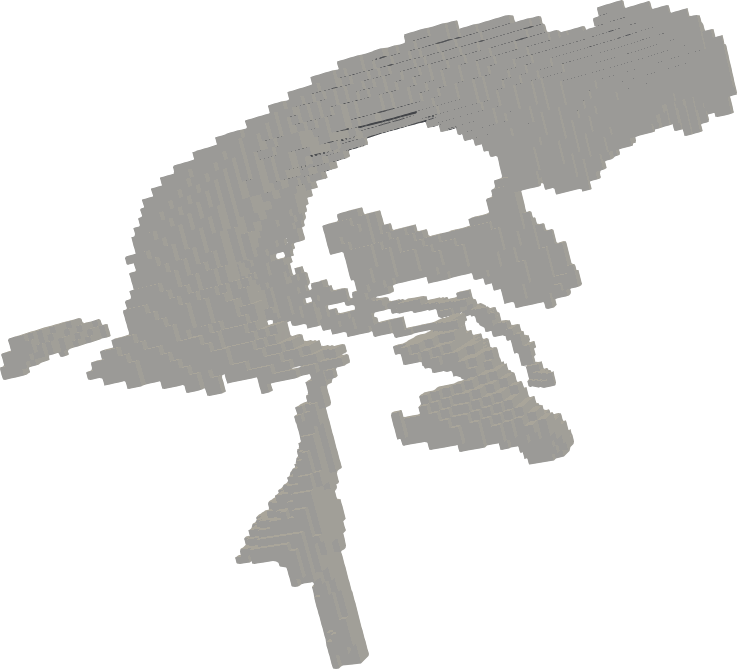
\includegraphics[width=0.49\textwidth]{./graphics/chp4/ernie-vent-0smooth-r.png}
  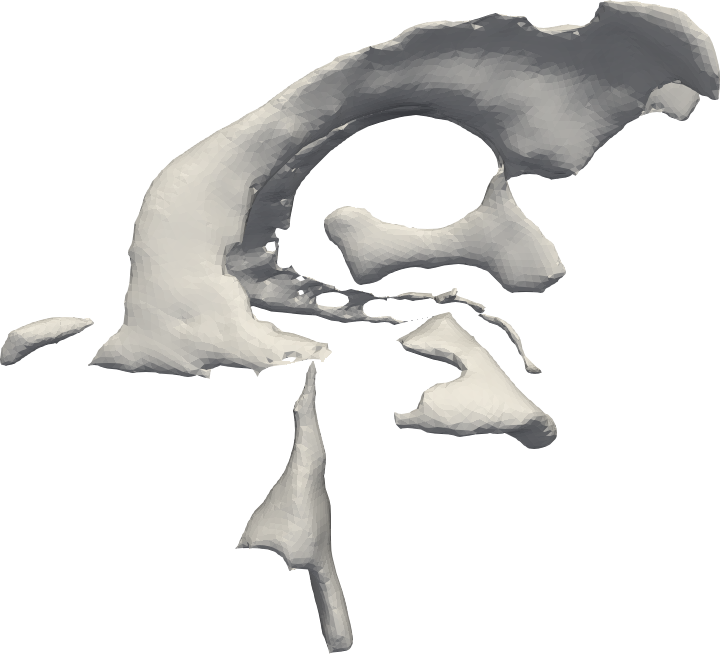
\includegraphics[width=0.49\textwidth]{./graphics/chp4/ernie-vent-5smooth-r.png}
  \caption{Ventricular surfaces, including the fourth ventricle,
    extracted and generated by \freesurfer{} from MRI images. No
    smoothing of the output surface (left) and five smoothing
    iterations (right). Note the disconnected regions.}
  \label{fig:chp4:ernie-ventricles-smoothing-example}
\end{figure}

In practice, the decision to include or discard the fourth ventricle
and aqueduct is data specific. The aqueduct may not be well resolved
in the MRI data on a patient-by-patient basis; if the aqueduct is not
visible in the data then keeping the fourth ventricle leads to a
ventricle system that is not connected, as
Figure~\ref{fig:chp4:ernie-ventricles-smoothing-example} indeed
shows. Moreover, if we include the fourth ventricle and aqueduct,
we should be cautious regarding the extent of the smoothing. 

\subsubsection*{Improving the morphology of the ventricular surface}
\index{connecting surfaces}
\index{FreeSurfer!\emp{mri\_volcluster}}
\index{FreeSurfer!\emp{mri\_morphology}}
In Section~\ref{sec:chp4:tools:remove-vent:removal}, we will use the 
ventricular surface to modify a volume mesh.  In this section, we discuss 
improving the ventricle surface by fixing a few morphological defects that may 
be present following the extraction process.  In particular, we will introduce 
the \freesurfer{} utilities \emp{mri\_volcluster} and \emp{mri\_morphology}.  
These tools can be used to: remove the smaller disconnected ventricle regions 
that may appear in the original surface extraction; close small holes in the 
large ventricle surface; and smooth the resulting surface before further use. 

\begin{itemize}
\item
  \emp{mri\_volcluster} is used to identify clusters in a volume. A
  cluster is defined as a set of continuous voxels that satisfies a
  specified volume threshold criteria; we will specify a minimum volume 
  threshold in the code example below. The input file is given following the 
  flag \emp{-{}-in}, \emp{-{}-thmin} gives a minimum threshold value,
  \emp{-{}-minsize} gives a minimal cluster volume (in
  mm$^3$). Different output flags are
  admissible~\cite{freesurfer-wiki}, including \emp{-{}-ocn}, used to
  save the output volume file with sorted clusters, where all voxels of
  the largest cluster will have the tag 1, the second largest would have
  the tag 2, and so on.
\item
  \emp{mri\_morphology} is used to perform certain operations on
  volume files and supports many operations.  These operations include opening, 
  closing, dilating, eroding and filling holes in a volume.  %We will 
  %illustrate how to use this function below for connecting the extracted 
  %domain by closing holes.
  We will make use of the `close' operation, of this utility, to close holes 
  in an extracted ventricle domain. 
\end{itemize}

Using these functions, we may extract an improved, higher-quality
ventricular surface by removing apparently disconnected regions. Our
algorithm takes the following steps:
\begin{enumerate}
\item
  We extract the lateral and third ventricles into a separate volume
  file.
\item
  In this separate volume, we extract clusters of connected voxels,
  but only those above a minimal cluster size. Since the average adult
  volume of cerebrospinal fluid in the ventricles is about 150
  mm$^{3}$, we set the threshold size to be around 100 mm$^3$.
\item
  We extract the largest of these clusters (thus ignoring smaller,
  disconnected regions)
\item
  We close any holes in the resulting volume as necessary.
\item
  We extract the surface of the resulting volume and smooth it as
  necessary.
\end{enumerate}
The corresponding continuation of our Bash script is as follows. Note
how we output the clusters sorted by size using the argument
\emp{-{}-ocn} to \emp{mri\_volcluster} and extract the largest
cluster by matching on one in the subsequent call to
\emp{mri\_binarize}. We allow for setting the number of closing
iterations \emp{num\_closing} and the minimal largest cluster size
\emp{V\_min} as parameters. We advise setting the number of closing
iterations relatively low (e.g.~to 1 or 2). Setting the number of closing
iterations too high can cause non-physiological connections in the
resulting ventricular surface.
\lstinputlisting[style=bashStyle,firstline=16,lastline=46]{../mri2fem/mri2fem/chp4/extract-ventricles.sh}

\begin{figure}%\sidecaption
  \centering
  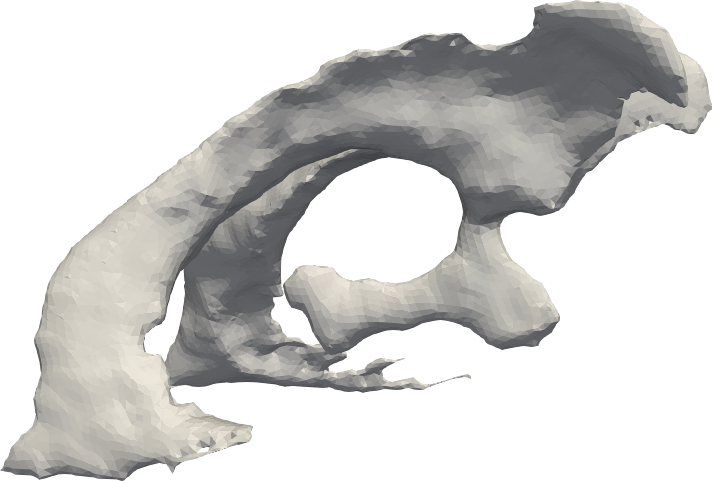
\includegraphics[width=0.75\textwidth]{./graphics/chp4/ernie-ventricles-final-r.png}
  \caption{Post-processed ventricle %High-quality, connected, smooth ventricular surface
    surface extracted from MRI using \freesurfer{}.  This surface file 
    (\emp{ernie-ventricles.stl}) is created by the script 
    \emp{mri2fem/chp4/extract-ventricles.sh}.}
  \label{fig:chp4:ernie-ventricles-final}
\end{figure}
\noindent Figure~\ref{fig:chp4:ernie-ventricles-final} shows the ventricular
surface STL file generated by the above code, with \emp{postprocess=true}, 
visualized in ParaView. 

\subsection{Removing the ventricular volume}
\label{sec:chp4:tools:remove-vent:removal}  
\index{SVM-Tk!\emp{Surface}}
\index{SVM-Tk!\emp{SubdomainMap}}
\index{SVM-Tk!\emp{remove\_subdomain}}
In this section, we demonstrate how to remove a subvolume defined by
an enclosing surface. Though we will focus, here, on removing the
volume enclosed by the ventricle surface, as extracted in the previous
section, the general process will also work for any volume defined by
a closed surface STL file. The core idea is to use \svmtk{} to
generate tags for the different subvolumes in the domain and then
simply delete the volume corresponding to a specific tag.  

We assume that we have the left pial, gray/white matter, and ventricular
surfaces available as STL files. Again, we will wrap the main
functionality in a Python function, called
\pythoninline{create\_gwv\_mesh}, to create the `gray matter plus white matter' 
volume mesh. This 
function can then, for instance, be called as
\newpythonsnippet{chp4}{three-domain-tagged.py}{33}{35}

\noindent This code example is included in
\emp{mri2fem/chp4/three-domain-tagged.py}.

We first create \pythoninline{Surface}s from the surface STL files:
\newpythonsnippet{chp4}{three-domain-tagged.py}{1}{10}

\noindent We then tag different regions using \pythoninline{SubdomainMap}: 
\newpythonsnippet{chp4}{three-domain-tagged.py}{12}{19}

\noindent As before, we create a tagged mesh (of a given resolution)
of the domain via the surfaces and the subdomain map:
\newpythonsnippet{chp4}{three-domain-tagged.py}{21}{24}

We can now, via a call to \svmtk{} \pythoninline{remove\_subdomain},
remove the mesh cells tagged as within the ventricles before saving
the mesh:
\newpythonsnippet{chp4}{three-domain-tagged.py}{26}{31}
Note that \pythoninline{remove\_subdomain} can also handle the removal of
multiple subdomains by providing a tuple of tags as input. The resulting
meshes, with and without ventricles removed, are shown in Figure
\ref{fig:chp4:tags-with-without-ventricles}.
\begin{center}
\begin{figure}
  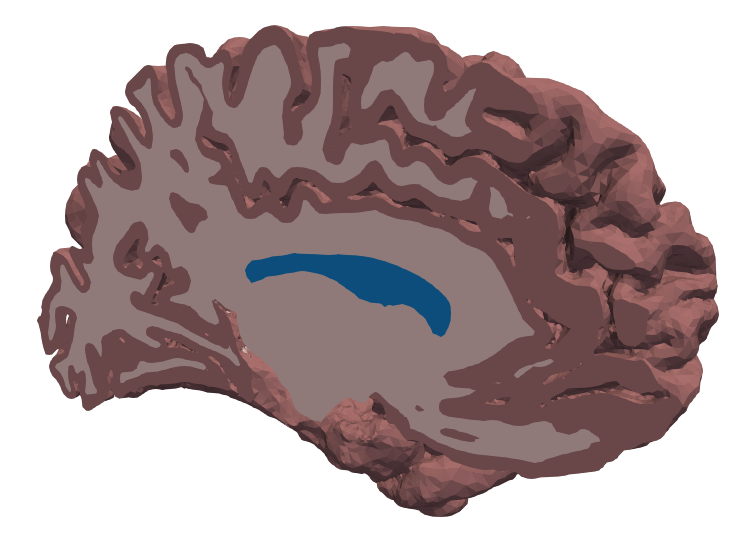
\includegraphics[width=0.49\textwidth]{./graphics/chp4/ernie-final-comp-b}
  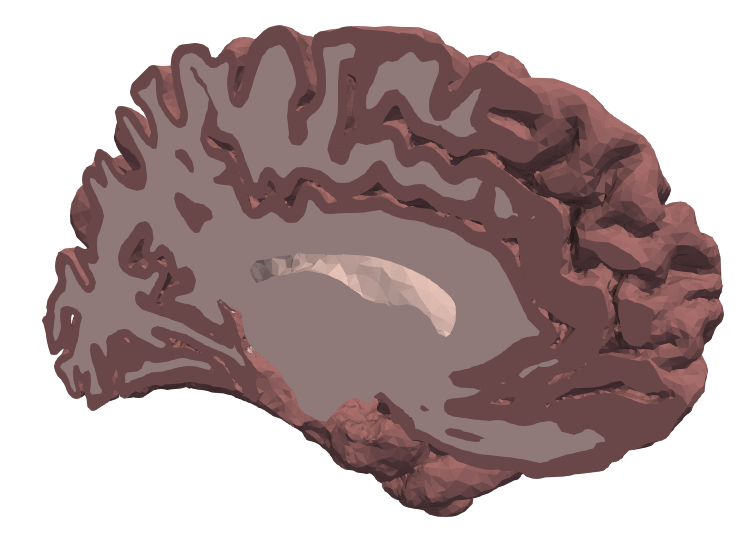
\includegraphics[width=0.49\textwidth]{./graphics/chp4/ernie-final-comp-d}
    \caption{Volume meshes of the left hemisphere (sagittal planes),
      conforming to the gray matter, white matter, and ventricles, with
      ventricles marked in blue (left) and with ventricles removed (right).  
	Note: that the tetrahedral boundary lines of the mesh have been 
	suppressed for visual clarity.  To view the tetrahedra of the mesh, 
	select the \emp{Surface With Edges} option, for the \emp{Representation} 
	setting in the left hand pane, after loading the \emp{.mesh} files, 
	created by \pythoninline{three-domain-tagged.py}, in ParaView. 
	}
    \label{fig:chp4:tags-with-without-ventricles}
\end{figure}
\end{center}

\section{Combining the hemispheres}
\label{sec:chp4-left-right-tagged}

In this section, our aim is to create a mesh that includes both the
left and right hemispheres, with gray and white regions tagged, and
the ventricular volume removed. We will combine the approaches of the
previous sections with \svmtk{} techniques for
working with the union of multiple surfaces. 

\subsection{Repairing overlapping surfaces}
\index{repairing surfaces}
\freesurfer{} generates the right and left hemisphere surfaces
separately. Combining surfaces from different hemispheres
can therefore create problems, such as
\begin{itemize}
\item The hemisphere surfaces overlap, creating bridges in the cortical gray 
matter, at the mesh and surface level, that do not exist physically.
\item The hemisphere surfaces may have gaps between them which are too large 
and are unphysical. In this case, the resulting mesh may undesirable gaps 
between the hemispheres where they would otherwise be connected by the 
white matter nerve tracts.  
\end{itemize} 
In general, we want to join the hemisphere surfaces, via the white matter 
nerve tracts, while simultaneously avoiding overlapping surfaces in the 
cortical gray matter.  %We can consider this a combined problem, since we 
%typically would want to join the hemisphere surfaces via the white matter 
% nerve tracts, while avoiding overlapping surfaces in the cortical gray matter. 
\svmtk{} includes utilities for addressing such challenges. In particular,
\begin{itemize}
\item
  \pythoninline{separate\_overlapping\_surfaces} can separate
  overlapping surfaces,
\item
  \pythoninline{separate\_close\_surfaces} can separate nearly-%
  overlapping surfaces, and
\item
  if we desire a single surface for the white matter but the white matter 
  surfaces only partially overlap, due for instance to smoothing, the 
  \svmtk{} function \pythoninline{union\_partially\_overlapping\_surfaces} 
  offers an improved set of features to handle the union operation of 
  the white matter surfaces.
%
%  if the surfaces partially overlap, due for instance to smoothing, and we 
%  want to create a single surface 
% 
%  if we want to create a single surface for the white matter but the
%  surfaces only partially overlap due to smoothing,
%  \pythoninline{union\_partially\_overlapping\_surfaces} offers
%  improved features to handle the union of white matter surfaces.
\end{itemize}
The following code snippet illustrates an example of the usage of these functions:
\begin{python}
# Input Surfaces
rpial = svmtk.Surface("rh.pial.stl")
lpial = svmtk.Surface("lh.pial.stl")
rwhite = svmtk.Surface("rh.white.stl")
lwhite = svmtk.Surface("lh.white.stl")

# Create white matter surface as union of hemispheres
white = svmtk.union_partially_overlapping_surfaces(rwhite,
                                                   lwhite)

# Separate overlapping and close vertices between
# the left and right pial surfaces,
# but only outside the optional third argument, which
# in this example is the white surface:
svmtk.separate_overlapping_surfaces(rpial, lpial, white)
svmtk.separate_close_surfaces(rpial, lpial, white) 
\end{python} 

\subsection{Combining surfaces to create a brain mesh}
We assume that left pial, left white, right pial, right white and
ventricular surface STL files have been extracted, converted and
possibly processed, by the processes described in the previous
section. Now, how do we combine these to create a complete brain mesh?

Again, we proceed via an \svmtk{} code example (with the complete
code included in \emp{mri2fem/chp4/fullbrain-five-domain.py}). We wrap
the main functionality in a Python function
\pythoninline{create\_brain\_mesh}. This function can then, for
instance, be called as:
\newpythonsnippet{chp4}{fullbrain-five-domain.py}{42}{45}

We begin by loading \emp{Surface}s from the STL files. 
\newpythonsnippet{chp4}{fullbrain-five-domain.py}{0}{7}
We take the union of the left and right white surfaces to illustrate
the possibility of combining surfaces:
\newpythonsnippet{chp4}{fullbrain-five-domain.py}{9}{15}
It is natural to ask whether we can do the same with the pial matter;
indeed, the union of the left and right pial surfaces is
possible. However, generally, whether one can successfully mesh the
joined surface, without further postprocessing, is data specific.
There is a higher chance that the {\freesurfer} segmentation process
of the left and right pial MRI surface data can lead to non-physical
intersections, thus producing left and right pial surface files that
overlap and self-intersect when combined.  Self-intersections within
a surface can then cause the meshing process to fail. Similarly, one
could simply work with all five surfaces separately.  This approach 
leads to a more complex tagging process, with \emp{SubdomainMap}, but
alleviates difficulties, such as the self-intersections mentioned above, 
that can arise when computing the union of two surface objects.

We continue by creating tags, a subdomain map, domain and mesh, and
leave the option of removing the ventricles, as in previous examples:
\newpythonsnippet{chp4}{fullbrain-five-domain.py}{17}{40} Note that
running this code example as is will take some time, on the order of a
few minutes. The resulting mesh can be visualized using ParaView
after conversion from .mesh to .vtu or .xdmf.

\section{Working with parcellations and finite element meshes} 
\label{sec:import-freesurfer-parcellation}
\index{parcellations}
{\freesurfer}'s \emp{recon-all} automatic segmentation process can identify 
almost two hundred different brain regions\footnote{{\freesurfer}'s \emp{recon-all} parcellates a brain into the regions 
defined by the Desikan-Killiany and Destrieux atlases.  Numbers are assigned 
to the different regions, by default, when \freesurfer{} performs the 
segmentation. These numbers are specific to \freesurfer{} but independent of a 
subject.  We note that the particular brain matter that \freesurfer{} 
identifies as `region N' (where N is some number) may differ between patients 
depending on their individual brain topology.}.  {\freesurfer} labels 
identified regions with a numeric code.  For instance, in the left 
hemisphere, \freesurfer{} assigns the numeric code of 17 to the 
hippocampus\footnote{In many
  neuroscience applications, the hippocampus region is of special
  interest because it is central to memory consolidation. The reader
  is refered to the interesting story of Henry Molaison, aka Patient
  H.M.,~\cite{squire2009legacy, scoville1957loss} who lost his ability
  to form new memories after the removal of both the left and right
  hippocampus. The procedure was performed as a treatment for his
  epilepsy. He lived for more than 50 years after the removal of his
  hippocampus and participated voluntarily in many scientific
  experiments, demonstrating the crucial role of the hippocampus. He
  never recognized the scientists who frequently visited him.}, 1035
to the gray matter insula, 3035 to the white matter insula, 1028 to
the gray matter superiorfrontal region and 3028 to the white matter
superiorfrontal region. Figure~\ref{fig:chp4:freesurfer-parc} (left) illustrates 
some of these regions using \emp{freesurfer/ernie/mri/wmparz.mgz} as an example. 
%
%An illustration of some of these regions,
%using \emp{freesurfer/ernie/mri/wmparz.mgz} as an example, is shown in
%Figure~\ref{fig:chp4:freesurfer-parc} (left).
%
\begin{figure}
\begin{center}
  \hspace{2em}
  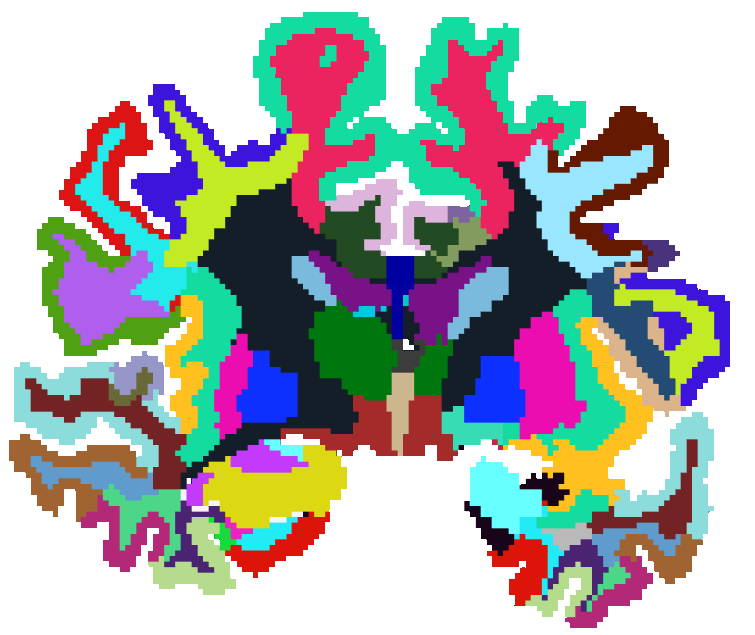
\includegraphics[height=4cm]{./graphics/chp4/parcellation-coronalwhiteBG_2.png}
  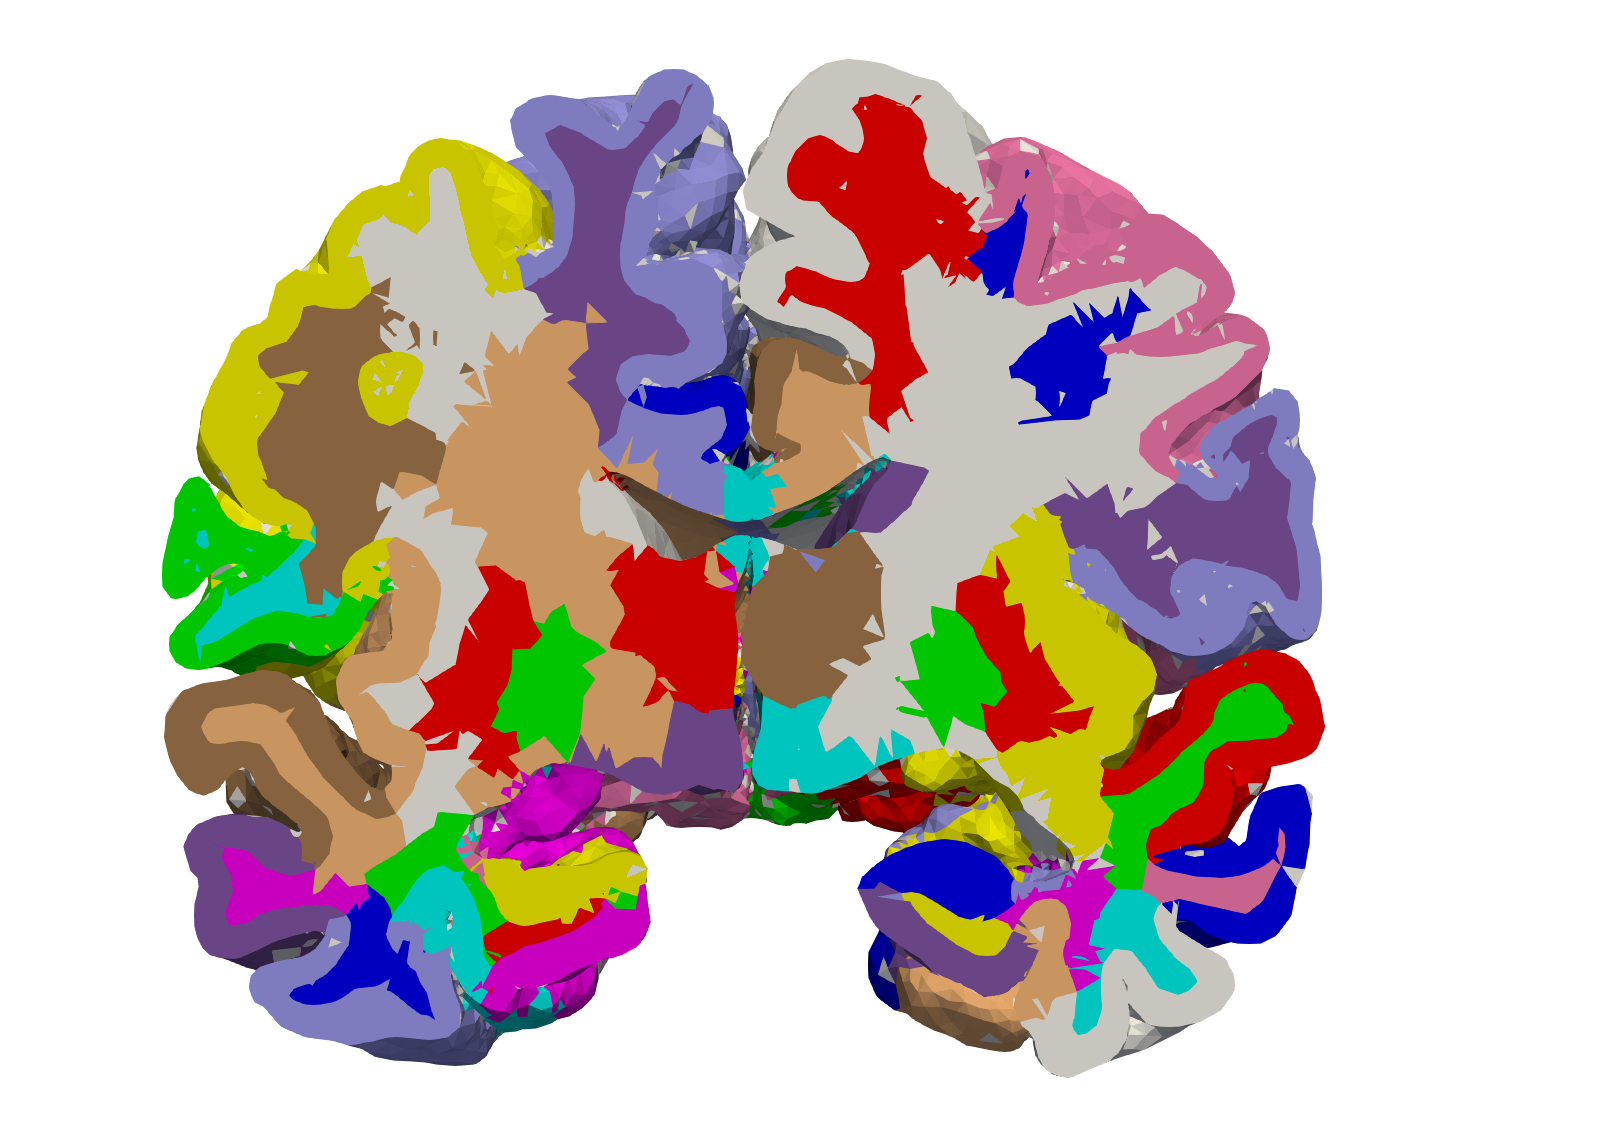
\includegraphics[height=4cm]{./graphics/chp4/ernie32-parcellation-basic.png}
  \caption{Brain parcellations: (left) as generated by \freesurfer{} and visualized 
   using Freeview and (right) the same parcellation transferred onto the {\fenics} 
   brain mesh and visualized using ParaView (with different colors, different 
   slices, and different view angles).} 
    %
    %Left: Parcellation as generated
    %by \freesurfer{} and visualized using Freeview. Right: Same
    %parcellation transferred onto the FEniCS brain mesh and visualized
    %using ParaView. (Different coloring, different slices, different view angles.)}
  \label{fig:chp4:freesurfer-parc}
\end{center}
\end{figure}

\subsection{Mapping a parcellation onto a finite element mesh}
\label{sec:chp4:mapping_parcellation}
\index{FEniCS}
In a brain parcellation, each region is identified by an integer
value. Our current goal is to map these region tags onto the
generated volume mesh and into a FEniCS-compatible format. Doing so
involves
\begin{itemize}
\item
  Reading and working with image (voxel-based) data in Python, 
\item
  Representing discrete mesh data in {\fenics},
\item
  Mapping values from voxel indices, namely, voxel space to mesh coordinates, %
  namely, left-to-right, posterior-to-anterior, inferior-to-superior (RAS) space.
\end{itemize} 
As usual, we will illustrate these steps using a concrete code example
(included in \emp{mri2fem/chp4/map\_parcellation.py}). We wrap our
main functionality in a Python function
\pythoninline{map_parcellation_to_mesh} taking the parcellation
filename and mesh filename as input (with \emp{wmparc.mgz} and
\emp{ernie-brain-32.xdmf} from the previous section as an example).
\newpythonsnippet{chp4}{map_parcellation.py}{64}{65}

\subsubsection*{Working with image data in Python}

\index{nibabel}
\index{FEniCS}
We will use the Python packages NiBabel to work %for working 
with neuroimaging data, NumPy for general numerics in Python, and {\fenics} to 
represent the mesh and the mesh data:
\newpythonsnippet{chp4}{map_parcellation.py}{1}{4}

\noindent We begin by loading the image data from the parcellation
file as follows:
\newpythonsnippet{chp4}{map_parcellation.py}{6}{10}

\noindent We can, for example, inspect the image shape (number of voxels in
each dimension) and extract voxel values by indexing the
\pythoninline{data} array:
\newpythonsnippet{chp4}{map_parcellation.py}{12}{16}

\subsubsection*{Representing discrete mesh data in FEniCS}
\index{FEniCS!\emp{MeshFunction}}
We aim to map the parcellation labels, generated by \freesurfer{} during 
segmentation, onto the brain mesh.  At this point, we have loaded a 
the \freesurfer{} \emp{wmparc.gz}; this parcellation was created from a 
set of T1 MR images.  We will also work with a mesh file; here, that 
file is \emp{ernie-brain-32.xdmf}.  This mesh file was generated from 
surfaces extracted from files which were also constructed, by \freesurfer{}, 
from a set of T1 images. We mention this because the following fact is 
important: to label a mesh file with parcellated region IDs, it is imperative 
that the T1 images used to generate the parcellation and the T1 images used 
to generate the mesh file are the same set of images. 
%
%We aim to map these labels onto the brain mesh generated from the same
%T1 images.


One way to associate discrete data, such as a parcellation label, with mesh 
elements is to use a {\fenics} \emp{MeshFunction}.
%FEniCS offers the concept of a \emp{MeshFunction} to represent such discrete 
%data.  
Mesh functions can be associated with geometrical objects, $X$, of various 
dimensions, $d = \text{dim}(X)$.  We can associate mesh functions with cells 
($d=3$), faces ($d=2$), edges ($d=1$), or vertices ($d=0$). Here, 
we aim to identify the parcellation region for each cell in the brain mesh and 
will thus make use of a cell function. We first import the full brain mesh:
\newpythonsnippet{chp4}{map_parcellation.py}{17}{21}

\noindent  Next, we create a mesh function for the mesh entities of dimension 
3 (tetrahedral mesh cells). Our \emp{MeshFunction} object will  
define a function whose input is a tetrahedron of the mesh and whose 
output, or associated value, is a real number; we start by specifying a 
mesh function associating an initial value of zero to all tetrahedrons of the 
mesh:  
\newpythonsnippet{chp4}{map_parcellation.py}{23}{27}
Note that the \emp{MeshFunction} can be indexed directly, or its values can be
accessed via the member function \emp{array}.

Our strategy, now, is: iterate over all cells in the mesh; identify the 
parcellation region label for each mesh cell; and set the associated value 
of the mesh function, for that cell, to the corresponding parcellation label 
value.  %
%We now aim to iterate this process over all cells in the mesh (function), 
%identify the corresponding parcellation region, and insert this value into 
%the \emp{regions} mesh function. 
However, at this point, a key question arises: While we can index the image's 
data by its indices and the mesh by its cell or vertex indices (and/or their 
coordinates), how can we identify the voxel index corresponding to a given 
cell or vertex (coordinate), and vice versa? 

\subsubsection*{Converting between indices, coordinates, and spaces}

\index{voxel space}
Converting between voxel indices and other coordinates is a core
problem that we will encounter several times. To address this task, we
begin by introducing some nomenclature. The span of the image
dimensions is often referred to as the (T1) \emph{voxel space}, with
indices (or dimensions) $(i, j, k)$. On the other hand, the span of
the mesh axes defines the RAS (left-to-\underline{r}ight, 
posterior-to-\underline{a}nterior, inferior-to-\underline{s}uperior) space 
with coordinates $(x, y, z)$. 

\index{FEniCS!HDF5}
We aim to
construct the transformation $f$ from voxel space to RAS space:
\begin{equation}
  (x, y, z) = f(i, j, k),
\end{equation}
as well as its inverse, $f^{-1}$, from RAS to voxel space. Fortunately,
the parcellation information allows us to extract this transformation easily:
\newpythonsnippet{chp4}{map_parcellation.py}{29}{33}

\noindent Note that FreeSurfer operates with several coordinate
systems, including different RAS spaces. In this book, RAS space will
refer to the FreeSurfer surface RAS space, which is identified
via the suffix \pythoninline{tkr} in the code snippet above.

Next, we iterate over the cells of the mesh.  For each cell, we will: 
extract the cell index; extract the RAS coordinates of the cell 
midpoint; convert from the RAS coordinates to voxel space (via a call to 
\emp{apply\_affine}); round off to the nearest integer values to find the 
image indices; and map the corresponding image data values into the 
\emp{regions} mesh function.  The code for this iterative process is
\newpythonsnippet{chp4}{map_parcellation.py}{35}{50}

We save the resulting mesh function in XDMF format (suitable for
ParaView) and in the HDF5 format (suitable for further FEniCS processing): 
\newpythonsnippet{chp4}{map_parcellation.py}{51}{62}
The result can be seen alongside the original parcellation in
Figure~\ref{fig:chp4:freesurfer-parc}.

\subsection{Mapping parcellations respecting subdomains}
\label{chp4:parcellations}

By careful inspection of the mesh-based representation of the
parcellation in Figure~\ref{fig:chp4:freesurfer-parc} (right), we find
some artifacts in the labeling of the cells. Indeed, since the finite
element mesh is not aligned with the segmentation, the previous direct
mapping between cell midpoints and voxels can lead to minor
inaccuracies. In this section, we therefore aim to improve on our mesh-based
parcellation representation by using subdomain
information. 


Concretely, we aim to do the following
\begin{itemize}
\item
  Read in a mesh with subdomain information.  The mesh may contain many 
  subdomains, such as those defined by a regional parcellation label.  The 
  mesh subdomain structure may also be simple, such as the gray / white matter
  subdomain regions discussed in~Section~\ref{sec:chp4:tools:gray-white:mesh-creation} 
\item
%  Iterate the process over the cells in each subdomain separately and calibrate
%  the voxel values against those of neighboring cells; and
  For each cell in every subdomain, determine if we should alter the label 
  assigned to the cell by inspecting the label of the neighboring cells 
\item
  Store the subdomain and parcellation information together.
\end{itemize}

\subsubsection*{Converting meshes and mesh data between different formats} 
\label{chp4:meshio-converting}

\index{meshio}
\index{FEniCS!\emp{Mesh}}
In Chapter~\ref{sec:chp4:tools:gray-white}, we created a mesh with
gray and white matter labels stored as subdomain information in the
.mesh format. Our next step is to convert this information to a
FEniCS-compatible format. We will write a convenient Python script for this
common operation and use the opportunity to illustrate the use of an
\pythoninline{ArgumentParser} to read in arguments from the command
line, instead of coding the arguments directly into the script
(included in \emp{mri2fem/chp4/convert\_to\_dolfin\_mesh.py}).

%We begin by importing the relevant Python packages, namely, \emp{argparse},
%\emp{meshio}, and \emp{dolfin}:
In this script, we will use the \emp{argparse} package to enable us to pass in 
command-line arguments that inform the conversion process.
\newpythonsnippet{chp4}{convert_to_dolfin_mesh.py}{1}{3}

\noindent Our argument parser set-up looks like this:
\newpythonsnippet{chp4}{convert_to_dolfin_mesh.py}{53}{59}
\noindent and we then  call two functions (described below): 
\newpythonsnippet{chp4}{convert_to_dolfin_mesh.py}{61}{63}
The script can then be called as, for example, 
\terminal{\$ cd mri2fem/chp4\\
\$ python convert\_to\_dolfin\_mesh.py -{}-meshfile ernie-gw.mesh -{}-hdf5file ernie-gw.h5}

We use meshio to first read the .mesh file, its data associated with
the mesh cells (\pythoninline{subdomains}), and its data associated with mesh
facets (\pythoninline{boundaries}). We then write these in the FEniCS-readable
.xdmf format as separate files.
\newpythonsnippet{chp4}{convert_to_dolfin_mesh.py}{5}{27}

Subsequently, {\fenics} can read the files \emp{mesh.xdmf} and \emp{subdomains.xdmf}, 
created above, into a \pythoninline{Mesh} object and \pythoninline{MeshFunction} 
object, respectively.  {\fenics} can then write the data from both objects 
into a single \emp{.h5} file:
%.xdmf files into a
%\pythoninline{Mesh} and \pythoninline {MeshFunction}s, and write these
%collectively to a single .h5 file:
\newpythonsnippet{chp4}{convert_to_dolfin_mesh.py}{29}{51}

%These can be read back into FEniCS as follows (with the filename 
%given in \pythoninline{hdf5file}):
The mesh, subdomain, and boundary information, saved above, can be read 
back into {\fenics} as follows (with the filename 
given in \pythoninline{hdf5file}):
\newpythonsnippet{chp4}{add_parcellations.py}{36}{46}

\subsubsection*{Masking data and improved parcellation identification}

Let us now assume that we have available the \emp{mesh},
\emp{subdomains}, as well as the image \emp{data} from the
parcellation file (e.g \emp{wmparc.mgz}) and the RAS to voxel space
transform \emp{ras2vox}, as described in
Chapter~\ref{sec:chp4:mapping_parcellation}. Our next steps are to
\begin{itemize}
\item
  Find the RAS coordinates of all cells (midpoints), and map these to
  voxel space indices and
\item
  Map parcellation values to mesh cells in a manner that ensures that the
  parcellation regions do not extend across subdomains.
\end{itemize}
In particular, for each mesh cell, we will now examine a neighborhood of the
corresponding voxel values to pick the most frequent adjacent one as
the matched parcellation value. 

We first extract all the RAS coordinates of the cell midpoints,
\newpythonsnippet{chp4}{add_parcellations.py}{57}{59}
before converting these to voxel coordinates and indices, as before:
\newpythonsnippet{chp4}{add_parcellations.py}{68}{72}

Now, we create two arrays.  The first array, \pythoninline{vox2sub}, provides 
a map from the index of a voxel to its subdomain tag;  the second array, 
\pythoninline{regions}, will hold the parcellation tags. 
%We create a convenient map from the voxel indices to the subdomain tags and
%the \pythoninline{regions} array to be filled:
\newpythonsnippet{chp4}{add_parcellations.py}{74}{81}

Now we adjust tags by a consensus method.  We do this by applying the following 
algorithm: for a fixed subdomain, iterate over the cells in that subdomain; 
for each cell, examine the voxel data (region label) associated to the neighbors 
of that cell but only those neighbors which also live in the same subdomain; set 
the region of the cell to the most common region of its neighbors.  This 
process is repeated for each subdomain in the mesh; the algorithm is 
implemented below: 
%
%We iterate the process over each subdomain separately, examine the voxel data
%associated with this subdomain only, and determine for each cell the most
%common tag in a neighborhood around its voxel:
%This algorithm is implemented below.
\newpythonsnippet{chp4}{add_parcellations.py}{83}{97}
We can then update the subdomain array
\newpythonsnippet{chp4}{add_parcellations.py}{99}{104}
and store the resulting mesh data again:
\newpythonsnippet{chp4}{add_parcellations.py}{106}{111}

The \pythoninline{adjacent_tag} function reads 
\newpythonsnippet{chp4}{add_parcellations.py}{7}{30}

The complete script is included in
\emp{mri2fem/chp4/add\_parcellations.py} and can be tested, for example, via 
\terminal{\$ python3 convert\_to\_dolfin\_mesh.py -{}-meshfile ernie-brain-32.mesh -{}-hdf5file ernie-brain-32.h5\\
  \$ python3 add\_parcellations.py -{}-in\_hdf5 ernie-brain-32.h5 -{}-in\_parc wmparc.mgz -{}-out\_hdf5 results/ernie-brain-subdomains-tags.h5 -{}-add 17 1028 1035 3028 3035
}

\section{Refinement of parcellated meshes}
\label{sec:chp4:addparcellations}
\index{mesh refinement!adaptive}
\index{FEniCS!\emp{refine}}
\index{FEniCS!\emp{adapt}}

We end this chapter by examining how we can refine the generated
meshes and, in particular, how we can refine local regions. FEniCS
supports global and local mesh refinement and adaptivity through the
functions \pythoninline{refine} and \pythoninline{adapt}. The latter
(\pythoninline{adapt}) is particularly useful for refining mesh
functions and associated mesh data, in addition to the refinement of
the mesh itself. The code snippets presented here are included in
a complete context in \emp{mri2fem/chp4/refine\_mesh\_tags.py}. 

\subsection{Extending the Python interface of DOLFIN/FEniCS}
DOLFIN, the problem-solving interface to FEniCS, provides a C++ and a
Python interface. The Python interface is generated from the C++
interface using pybind11, but the entire C++ API is not
exposed. Instead, a user can generate their own Python bindings fairly
easily. Since parts of the \pythoninline{adapt} interface are not, by
default, available in Python, we illustrate how to use pybind11 to
compile our own FEniCS wrappers here.

We provide Python bindings for the \emp{adapt} function as follows: 
\newpythonsnippet{chp4}{refine_mesh_tags.py}{4}{18}

We also notice that this function is overloaded, and we provide
bindings to three versions with different signatures. After the code is
executed, the bindings are compiled by the Python module. However,
note that the module will not be added to the DOLFIN library, but
resides in the user's local cache.

\subsection{Refining certain regions of parcellated meshes}
It may be desirable to refine a mesh; either globally or within particular 
regions.  In this section, we discuss two options for refinement; global and 
local.  The code snippets in this section can be found in the file 
\pythoninline{refine\_mesh\_tags.py}.  Let us assume that, 
in Python, we have a FEniCS \emp{mesh} with FEniCS mesh functions 
\emp{subdomains} and \emp{boundaries}, for instance, extracted from an .h5 file, 
as illustrated in Chapter~\ref{chp4:parcellations}. 

One option is, then, to refine the mesh globally, meaning that we refine
all the cells of the mesh. We would then also like to refine or adapt the
associated mesh functions to the refined mesh. We can accomplish this
as follows:
\newpythonsnippet{chp4}{refine_mesh_tags.py}{35}{48}

\begin{figure}[t]	
  \begin{center}
    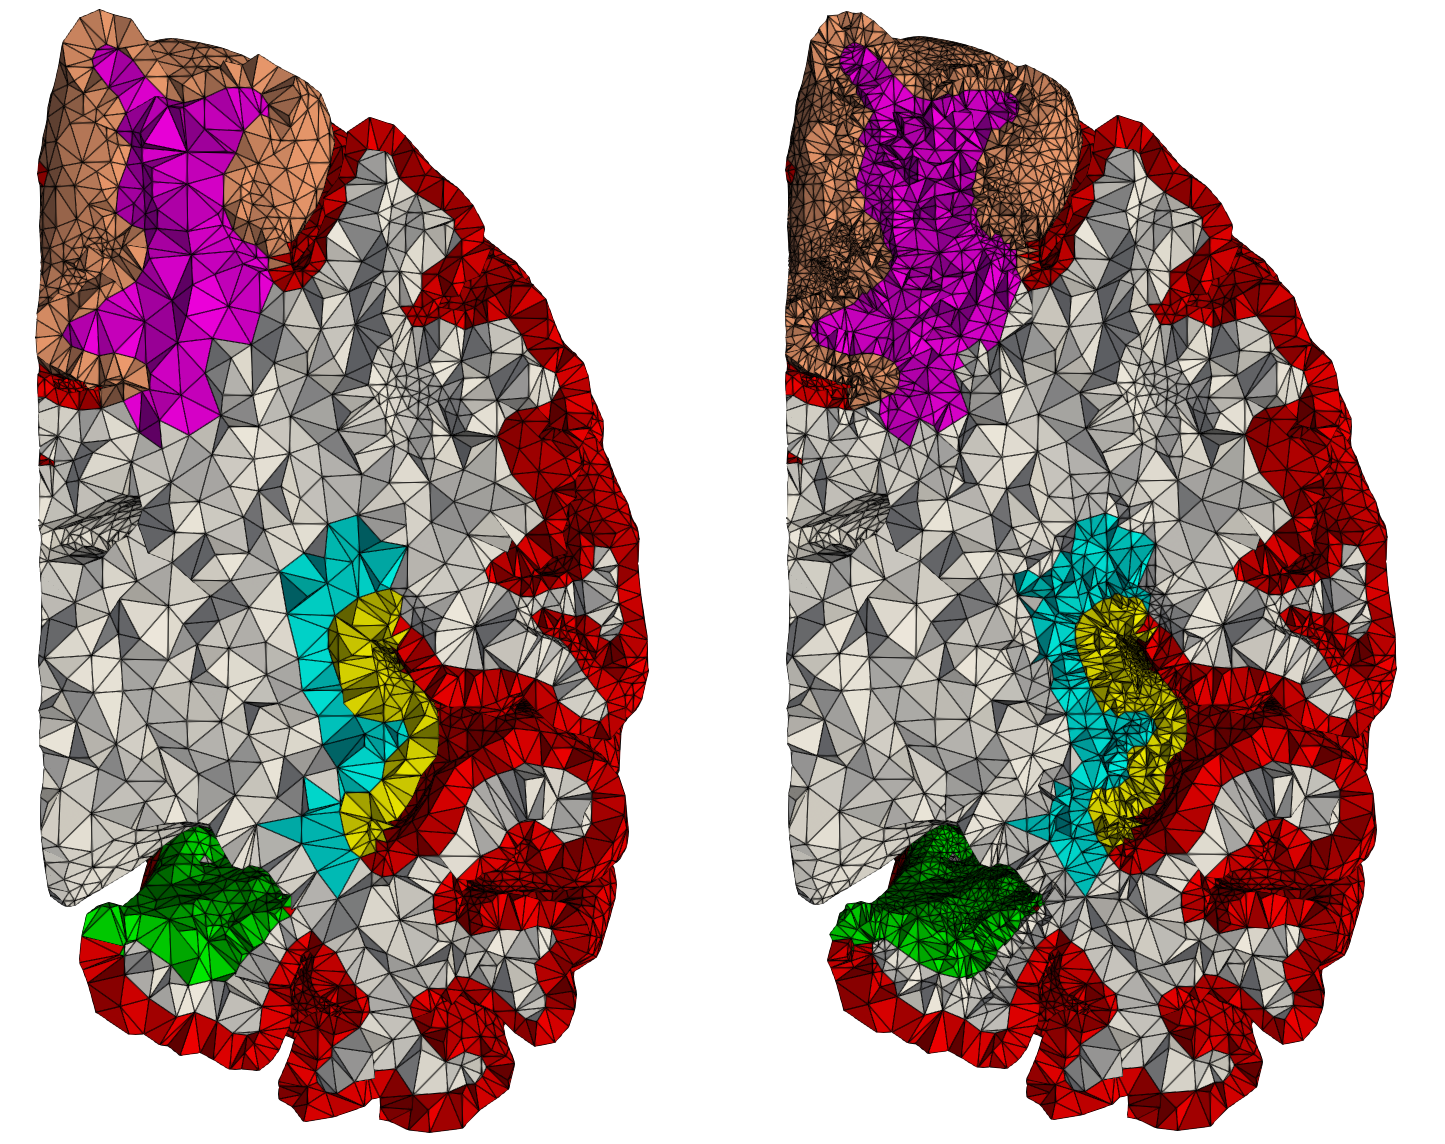
\includegraphics[width=0.7\textwidth]{./graphics/chp4/fenics-parcellation-crinkle.png} \\
    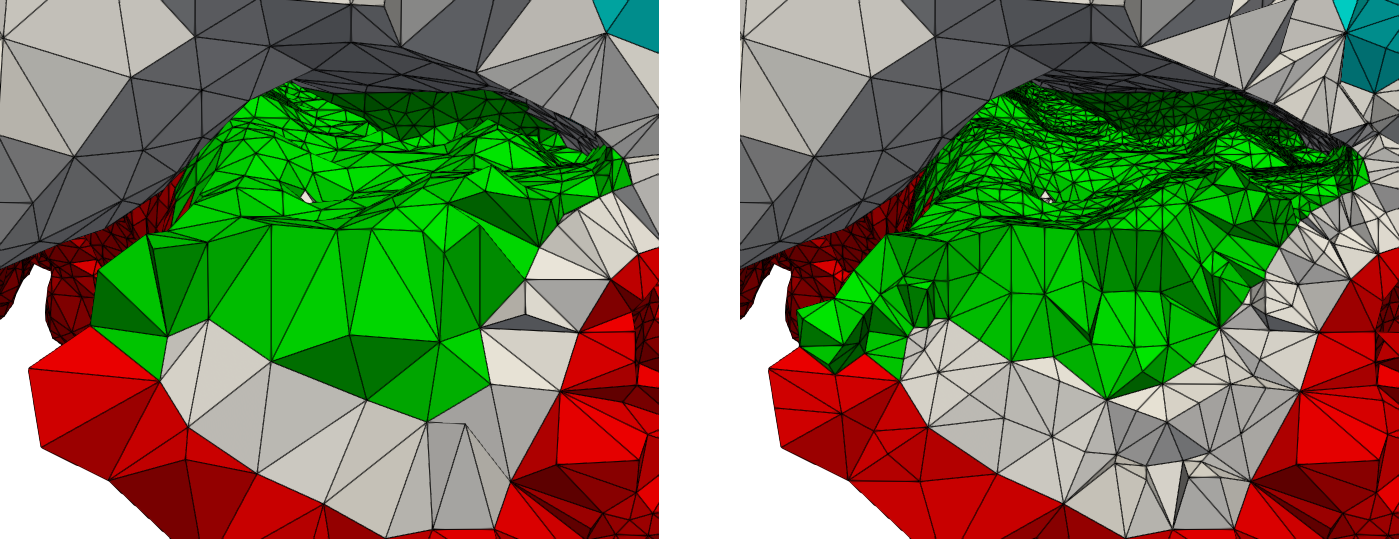
\includegraphics[width=0.9\textwidth]{./graphics/chp4/parcellations_refine_zoom.png}
  \end{center}
  \caption{Illustration of a locally refined left hemisphere mesh.  The left 
  figures show the original mesh with labeled (color coded) regions.  The 
  right figures show the locally refined mesh.  Only particular 
  regions have been refined; compare the green region to the red region.  Local 
  refinement is carried out using \pythoninline{refine\_mesh\_tags.py} and 
  using the \emp{-{}-refine\_tag} option.}
%
    %The meshes on the
    %right are local refinements of the meshes on the left. Zoomed in view of 
    %the hippocampal region (green).  Note that some regions (red, for instance) 
    %are not refined}
  \label{fig:chp4:fenics-parc}
\end{figure}
Notice that the script \pythoninline{refine\_mesh\_tags.py} refines the mesh 
globally if the \pythoninline{tags} is empty.  The \pythoninline{tags} list 
can be specified, or not, as an input argument to 
\pythoninline{refine\_mesh\_tags.py}.  For global refinement, we do not want 
to specify tags; the following command will globally refine the mesh, 
\emp{ernie-brain-32.h5}, created in the previous section:

\terminal{\$ python3 refine\_mesh\_tags.py -{}-in\_hdf5 ernie-brain-32.h5 -{}-out\_hdf5 ernie-brain-32-refined.h5}

%Alternatively, we can refine the mesh locally. To do so, we
%provide the adapt function with a Boolean cell-based mesh function
%that sets each mesh cell as a candidate for refinement (\emp{True}) or
%not -- unless as a side effect of the refinement algorithm
%(\emp{False}). Assuming that we have a list \emp{tags} with the
%subdomain tags for parcellation regions that we would like to
%refine, we consider the following:
Alternatively, we can refine the mesh locally.  In the code, this is done by 
providing the \emp{adapt} function with a Boolean cell-based mesh function
that sets a value of \emp{True} or \emp{False} at each mesh cell 
(i.e.~tetrahedron).  A value of \emp{True} indicates that the cell should be 
refined while \emp{False} indicates it should not.  The code starts by setting 
every cell's associated value to \emp{False}.  Then, we loop over the mesh 
cells and check to see if the cell's region matches a region in the 
\pythoninline{tags} list; if so, we mark this cell for refinement by changing 
its associated value to \emp{True}.  The relevant code snippet is: 
\newpythonsnippet{chp4}{refine_mesh_tags.py}{50}{64}

In practice, the \pythoninline{tags} list 
is populated by passing in command line arguments to the script.  For instance, 
the following command will refine the cells in regions 17 (left hippocampus), 
1028 (left superior frontal cortex), 1035 (left insular cortex), 3028 (left 
superior frontal white matter) and 3035 (left insular white matter).

\terminal{\$ python3 refine\_mesh\_tags.py -{}-in\_hdf5 ernie-brain-32.h5 -{}-out\_hdf5 ernie-brain-32-refine-tags.h5 -{}-refine\_tag 17 1028 1035 3028 3035}

We remind the reader that the various tags can be found by opening Freeview 
(c.f.~Chapter~\ref{sec:chp2:software-ecosystem}), selecting 
\button{File$\rightarrow$Load Volume} from the top menu, selecting 
\emp{mri2fem/chp4/wmparc.mgz}, and then setting the \emp{Color map} option (in 
the left pane) to \emp{Lookup Table}.  The local refinement of a mesh with 
labeled parcellation regions is illustrated in 
Figure~\ref{fig:chp4:fenics-parc}.



